\documentclass[a4paper, 12pt, titlepage]{article}
%=======Unpackage Things===============
\usepackage{array}
\usepackage{color}
\usepackage{colortbl}
\usepackage{float}

\usepackage{graphicx}
\usepackage{amsmath}
\usepackage{amsthm}
\usepackage{listings}
%\usepackage{fullpage}
\usepackage{epsfig}
\usepackage{latexsym}
\usepackage{amssymb}
\usepackage{amstext}
\usepackage{enumerate}
\newcommand{\PreserveBackslash}[1]{\let\temp=\\#1\let\\=\temp}
\newcolumntype{C}[1]{>{\PreserveBackslash\centering}p{#1}}
\newcolumntype{R}[1]{>{\PreserveBackslash\raggedleft}p{#1}}
\newcolumntype{L}[1]{>{\PreserveBackslash\raggedright}p{#1}}


\begin{document}
\section{Linear and Polynomial Regression}
\begin{enumerate}[(a)]
        \item Load traning set and plot 
            \begin{figure}[H]
                \centering
                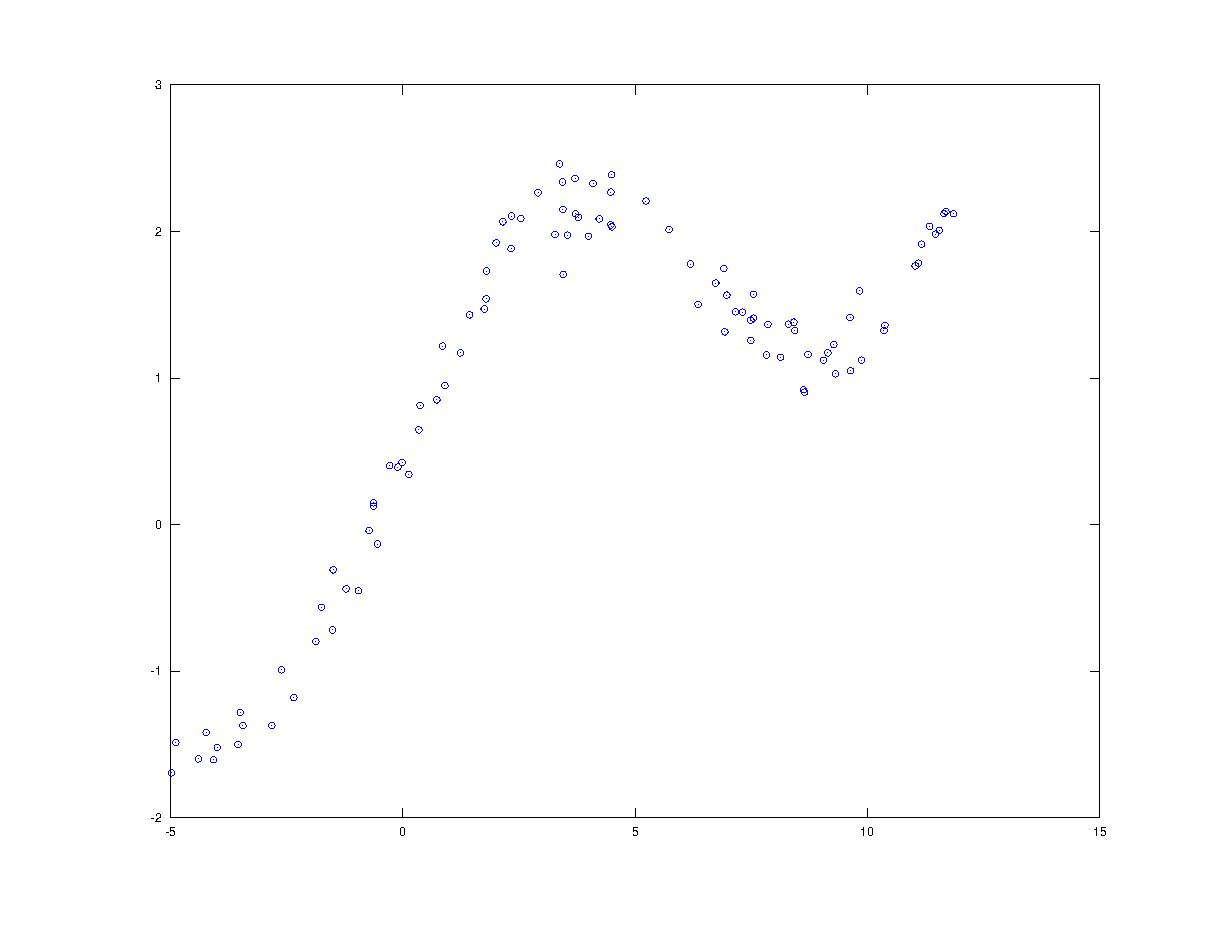
\includegraphics[width=8cm]{fig/a.eps}
                \caption{Plot Training Set}\label{a}
            \end{figure}
        
        \item Add a column of 1s and perform linear regression
            \begin{figure}[H]
                \centering
                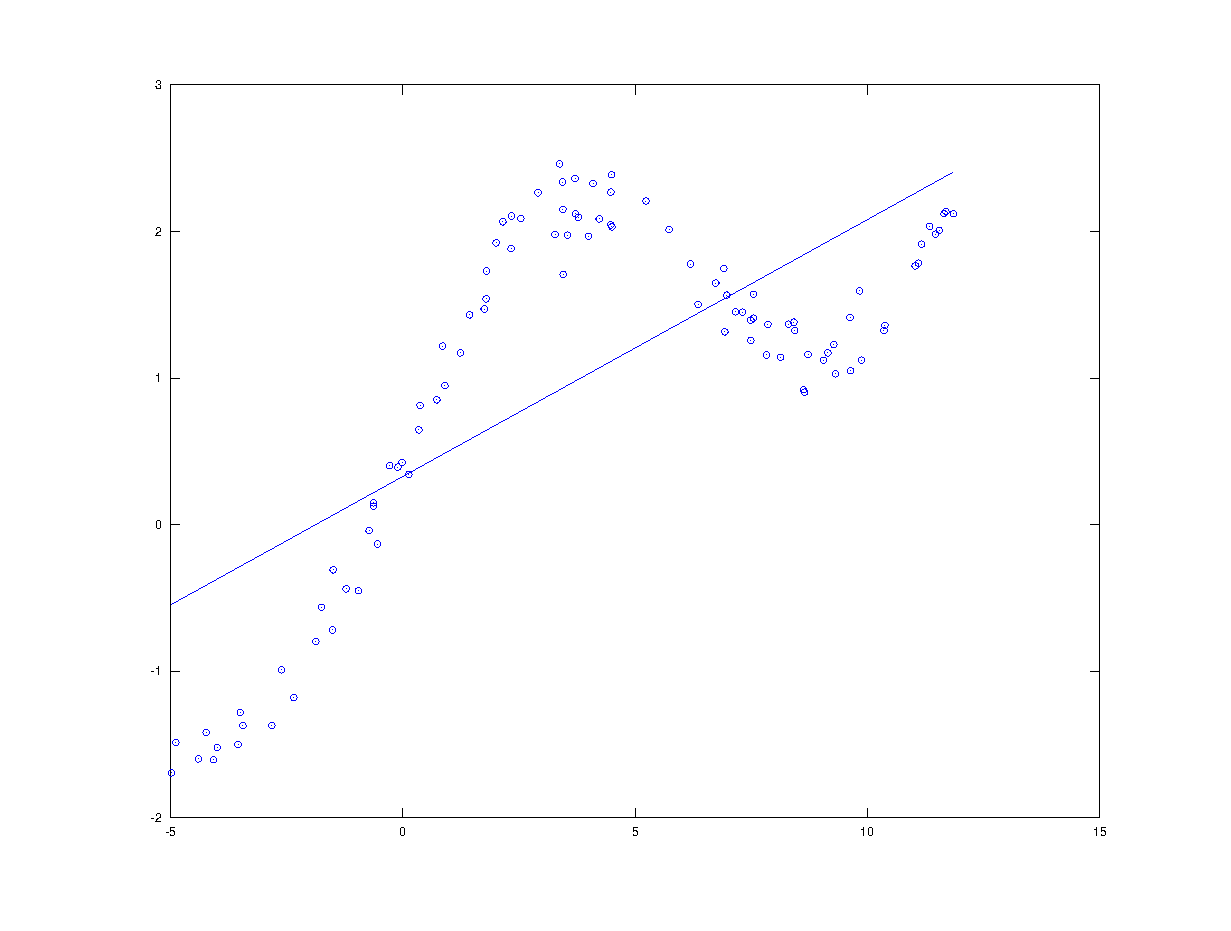
\includegraphics[width=8cm]{fig/linear.eps}
                \caption{Linear Regression}\label{b}
            \end{figure}

        \item The error function I used is \emph{sum-of-squares} function.
            $$J(w)=\frac{1}{2}\sum^m_{i=1}(h_w(x_i)-y_i)^2$$
            The function is implemented in J.m, which takes X, Y and W as parameters.

            The error of linear regression is 33.336445.
        \item The polynomial regression is implemented in PolyRegress.m
        \item Quadratic regression
            \begin{figure}[H]
                \centering
                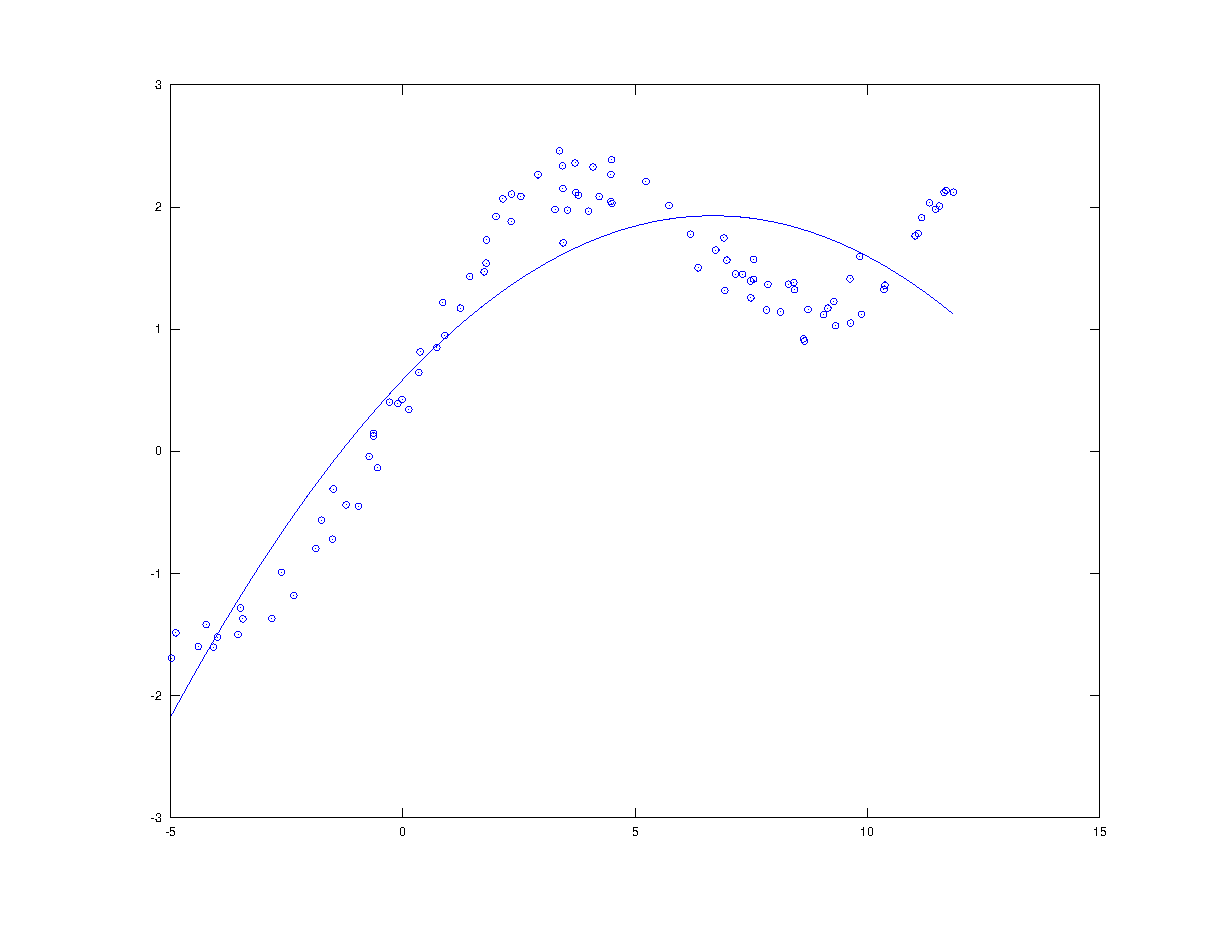
\includegraphics[width=8cm]{fig/quad.eps}
                \caption{Quadratic Regression}\label{e}
            \end{figure}

            error = 12.613

            Obviously, it is a better fit than linear regression.

        \item Cubic Regression %(f)
            \begin{figure}[H]
                \centering
                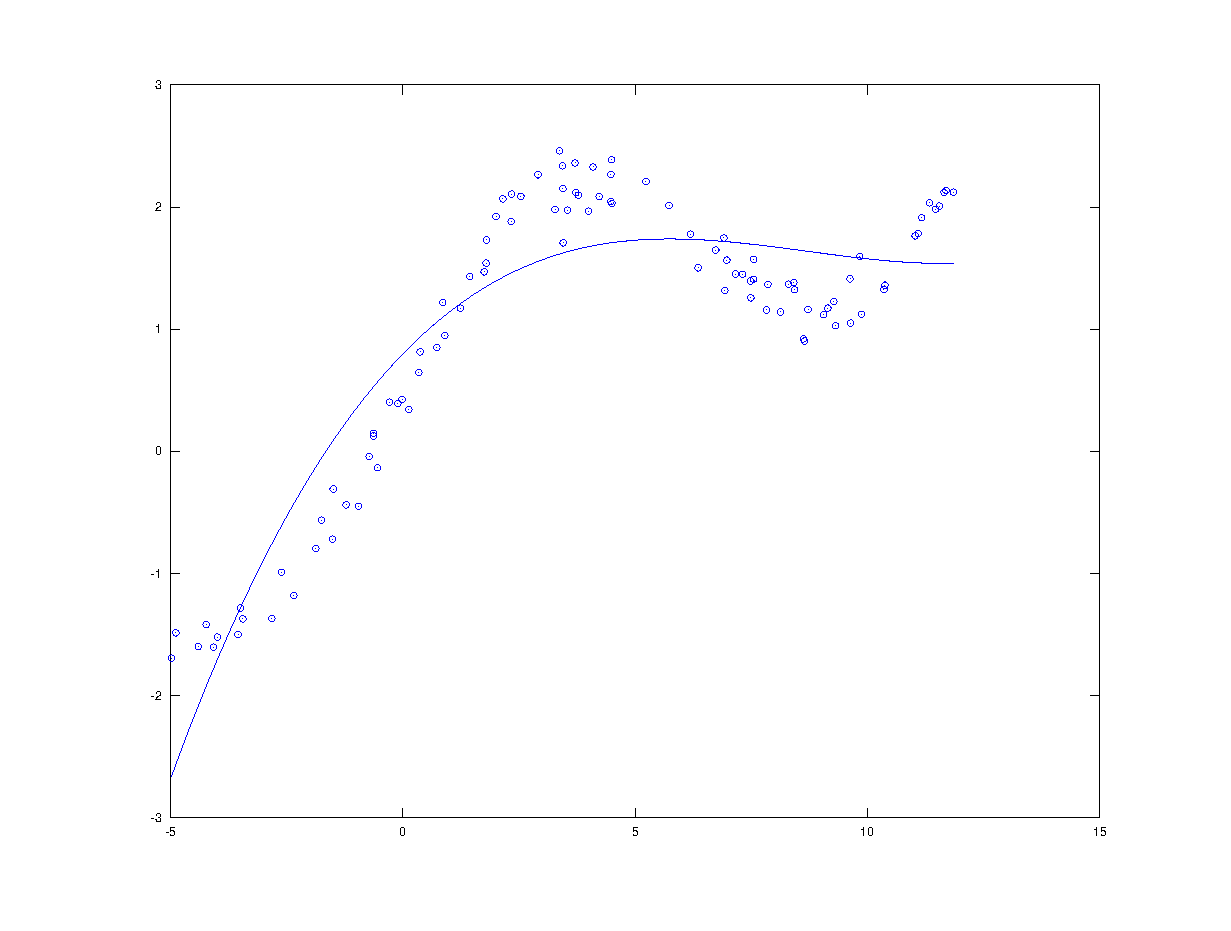
\includegraphics[width=8cm]{fig/cubic.eps}
                \caption{Cubic Regression}\label{f}
            \end{figure}

            error = 10.878

            Comparing with the cubic regression, it is a better fit.

        \item %(g) 

        \item %(h)


\section{Weighted Linear Regression}
            

\end{enumerate}
\end{document}
